\documentclass[10pt,twocolumn]{article}

\usepackage[left=0.25in,right=0.25in,top=0.25in,bottom=0.25in]{geometry}
\usepackage{amsmath,amsfonts}
\usepackage{graphicx}
\usepackage{hw}
% \usepackage{multicol}

\setlength{\parindent}{0pt}

\graphicspath{ {.} }


\begin{document}
% \begin{multicols}{2}

\section{Frequent pattern mining}
Transaction Database: 
Absolute support (count): $sup\{X\}$; Relative support (fraction): $s\{X\}$.

Compute the confidence of association rule $X\rightarrow Y$:\\ 
$x=sup(X,Y)/sup(x)$ (form $X\rightarrow Y (s,c)$)

\textbf{Apriori:} Downward closure (any subset of frequent item is frequent). Steps: 1. find the complete set of frequent k-itemsets; 2. derive frequent (k+1)-itemset candidates; 3. Scan DB again to find true frequent (k+1)-itemsets (via self-joining; pruning). It's \textbf{breadth-first} search.  

\textbf{FP-growth}: depth-first search (subsequent search confined to those with specific itemset). Steps: Order frequent list and insert into FP-trees. 
Mine (conditional) FP-trees: single path generate all the combinations of its sub-paths.

\begin{figure}[!ht]
    \centering
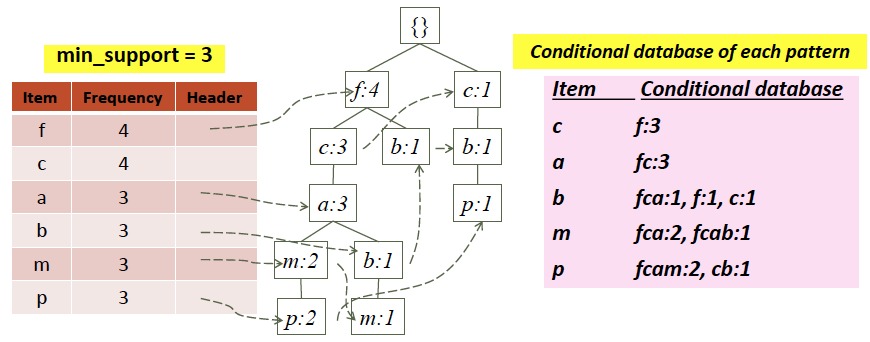
\includegraphics[width=0.6\linewidth]{fig/FPG.png}
\end{figure}

\textbf{Pattern Evaluation:} \\
% Interestingness measure: 1. $lift(B,C)=\frac{c(B\rightarrow C)}{s(C)}=\frac{s(B\cup C)}{s(B)\times s(C)}$. If $lift>1$, positive; otherwise, negative\\
% 2. $\chi^2=\sum\frac{(observed-expected)^2}{expected}$. Check confidence by $\chi^2$ table. If expected>observed, negative.

\begin{figure}[!ht]
    \centering
    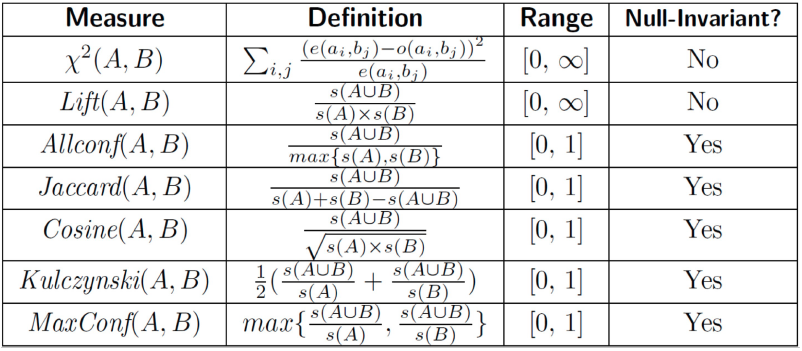
\includegraphics[width=0.8\linewidth]{fig/interestMeasure.png}
\end{figure}

Imbalance ratio: $IR(A,B)=\frac{|s(A)-s(B)|}{s(A)+s(B)-s(A\cup B)}$

Lift and $\chi^2$ are good measures if null transactions are not predominant. Otherwise, Kulczynski + Imbalance Ratio. 

\textbf{Sequential Pattern}: \\
Sequence: e.g.$<(ef)(ab)cb>$; Note: unordered in (..)
\begin{figure}[!ht]
    \centering
    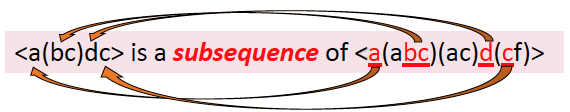
\includegraphics[width=0.6\linewidth]{fig/seq_pattern.png}
\end{figure}

\textbf{GSP}: apriori-based sequential pattern mining.
Steps: 1. generate initial candidates (singleton); 2. scan and count support; 3. generate length-2 candidates (ordered+unordered: n*n+n(n-1)/2) 

\textbf{SPADE}: A sequence database is mapped to: $<SID, EID>$; Grow the subsequences (patterns) one item at a time by Apriori candidate generation

\textbf{Prefix-span:} Pros: No candidate subseqs. to be generated; Projected DBs keep shrinking; Cons: Suffixes largely repeating in recursive projected DBs (solution: pseudo-projection+Physical Projection (DB not fit in memory))
\begin{figure}[!ht]
    \centering
    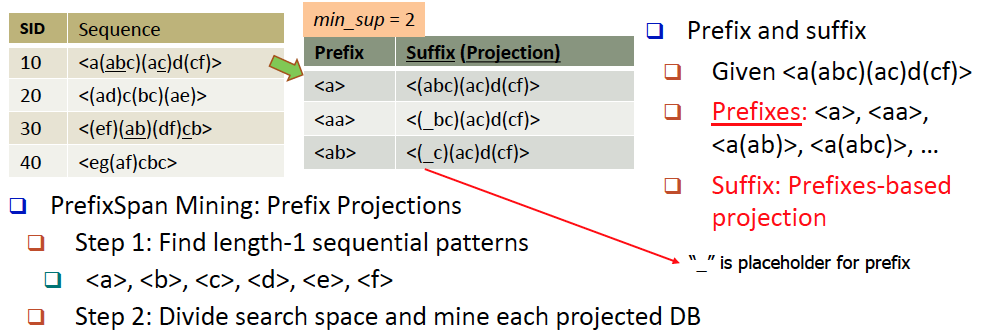
\includegraphics[width=0.8\linewidth]{fig/spade.png}
\end{figure}

\textbf{Graph Pattern}: 
% Given a labeled graph dataset $D=\{G_1, G_2,\dots, G_n\}$, the supporting graph set of a
% subgraph g is $D_g={G_i|g\subseteq G_i, G_i\in D}$. $support(g)=|D_g|/|D|$
Apriori-based method: Breadth-search, Apriori joining two size-k graphs. With one more vertex: AGM; with one more edge: FSG. 

Pattern-Growth Approach: Depth-first growth of subgraphs from k-edge to (k+1)-edge. Limits: Generating many duplicate subgraphs; Solutions: Define an order to generate subgraphs; DFS spanning tree: Flatten a graph into a sequence using depth-first search; \textbf{gSpan}: Right-most path extension; Backward extension (b-c) vs. forward extension (d-g)
\begin{figure}[!ht]
    \centering
    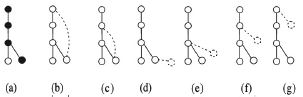
\includegraphics[width=0.5\linewidth]{fig/gspan.png}
\end{figure}
DFS code: $(i; j; l_i; l_{(i;j)}; l_j )$, $l_i$ is vertex label, and $l_{(i;j)}$ is edge label.

\section{Classification}
\textbf{Feature selection:} remove irrelevant and redundant features. How to construct? Domain knowledge or deep learning. 

Methods: 
filter methods (based on goodness measure, independent of classification model): fisher scores:
$s=\sum_{j=1}^cn_j(\mu_j-\mu)^2/\sum_{j=1}^c n_j\sigma_j^2$; $\chi^2$ test; information gain; mutual information.

wrapper methods (combine feature selection and classification model iteratively): exhaustive search ($2^p-1$); stepwise forward selection; stepwise backward elimination; hybrid method

Embedded methods (simultaneously construct classification model and select features): \textbf{LASSO} \\
Model $\hat{L}(w)=\frac{1}{2}\sum_{i=1}^n(y_i-\hat{y}_i)^2+\lambda\|w\_1\|=\frac{1}{2}\sum_{i=1}^n(y_i-w^Tx_i)^2+\lambda \sum_{j=0}^d|w_j|$ (goodness of prediction+(convex) approximation of \# of selected features). Training: coordinate descent (for $f(x)=g(x)+\sum_ih_i(x_i)$, if f(x) is convex but not differential, but separable (g(x) is convex and smooth; $h_i(x)$ is convex) $\rightarrow$ global minima). 

Training: update on $w_t$ while fixing others. \\
$\beta_t=argmin_{w_t}\frac{1}{2}\sum_{i=1}^n(r_i-w_tx_{i,t})^2$ and $r_i=y_i-\sum_{j=0,j\neq t}^dw_jx_{i,j}$ 
Then solve the optimization problem: $L(w_t)=\frac{1}{2}(w_t-\beta_t)^2+\lambda|w_t|$, assume each feature is normalized: $x_t^Tx_t=\|x_t\|^2=1$. \textbf{Solution}: soft-thresholding (intuition: push $\beta_t$ toward 0)
\begin{figure}[!ht]
    \centering
    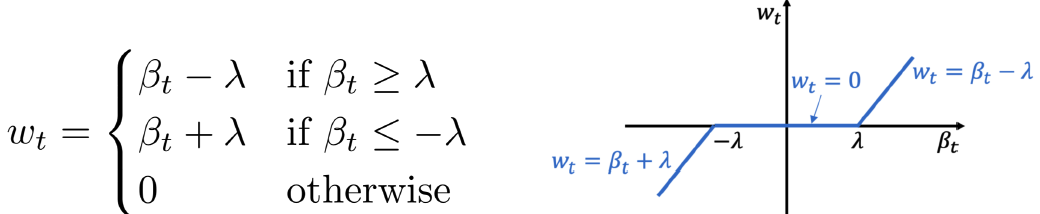
\includegraphics[width=0.6\linewidth]{fig/coord_descent.png}
\end{figure}

\textbf{SVM}\\
Reasons of distorted boundaries: irregular distribution, imbalanced training size, outliers. 

Maximum margin classification: margin $m=\frac{2c}{\|w\|}$. Optimization: $max_{w,b}\frac{1}{\|w\|}\ s.t\ y_i(w^Tx_i+b)\ge1,\forall i \Leftrightarrow min_{w,b}\frac{1}{2}w^Tw\ s.t\ 1-y_i(w^Tx_i+b)\le0,\forall$. Then write Lagrangian: $L(w,b,\alpha)=\frac{1}{2}w^Tw-\sum_{i=1}^m\alpha_i[y_i(w^Tx_i+b)-1]$ for $max_{\alpha_i\ge0}min_{w,b}L(w,b,a)$.

\textbf{Dual opt problem}:
$max_\alpha L(\alpha)=\sum_{i=1}^m\alpha_i-\frac{1}{2}\sum_{i,j=1}^m\alpha_i\alpha_jy_iy_j(\mathbf{x}_i^T\mathbf{x}_j)\ s.t\ \alpha_i\ge0,\sum_{i=1}^m\alpha_iy_i=0$

After solving it, $w=\sum_{i=1}^m\alpha_iy_i\mathbf{x}_i$: linear combination of small number of data points (sparsity). To compute $\alpha_i$, specify inner products between examples ($\mathbf{x}_i^T\mathbf{x}_j$). Prediction: $y^*=sign(\sum\alpha_iy_i(\mathbf{x}_i^Tz)+b)$

Kernels for non-linear classifier: $K(x,x')=\phi(x_i)^T\phi(x_j)$. Linear kernel: $x^Tx'$; polynomial kernel: $(1+x^Tx')^n$; radial basis kernel: $exp(-\frac{1}{2}\|x-x'\|^2)$

\textbf{Soft-margin SVM}: \\
$min_{w,b}\frac{1}{2}w^Tw+C\sum_{i=1}^m\xi_i,\ s.t\ y_i(w^Tx_i+b)\ge1-\xi_i, and\ \xi_i\ge0, \forall i$, where $\xi_i$ is slack variable which approximiates the numebr of misclassified samples. C: balance error and margin. The dual form: $max_\alpha L(\alpha)=\sum_{i=1}^m\alpha_i-\frac{1}{2}\sum_{i,j=1}^m\alpha_i\alpha_jy_iy_j(\mathbf{x}_i^T\mathbf{x}_j),s.t\ 0\le\alpha_i\le C\ and \sum_{i=1}^m\alpha_iy_i=0$

SMO algorithm: coordinate ascend. 1. Select some pair $\alpha_i$and $\alpha_j$ to update next; 2. reoptimize $J(\alpha)$ w.r.t $\alpha_i$ and $\alpha_j$ while holding others fixed. 

LR as unconstraint opt problem: $argmin_{w,b}w^tw+\lambda\sum_{i=1}^m(ln(1+exp(-w^Tx_i))+(1-y_i)w^Tx_i)$.

\textbf{Weakly-supervised learning}\\ 
SSL: self-training: use classifier to label unlabeled data; co-training: f1 and f2 on two separate feature sets; classify unlabeled data; add most confident $(x, f_1(x))$ to labeled dataset of f2, etc.
SSL assumption: cluster assumption: Data tuples from same cluster are likely to share same label; manifold assumption:  A pair of close tuples are likely to share the same class label. 

Transductive learning: unlabeled data appeared in test (no test data)

Active learning: find best unlabeled data to ask oricle (human involved). Key: how to choose? Uncertainty sampling; query-by-committee; version space; decision-theoretic approach.

Transfer learning: transfer most relevant/similar data from source to target. Challenge: negative transfer (quantify difference between source and target; transfer margin, divergence metric)

Distance supervision: challenge: noisy but large in volume 

Zero-shot learning: predict test tuple not observed in training. Semantic attribute classifier: train and use semantic attribute classifier to infer semantic attributes and use them to predict novel class. 

Stream data classification: challenge: high arrival speed (use most recent chunk); infinite length; one-pass constraint (Each incoming data is accessed once to train classifier and update weights of each classifier); concept drifting (adjust weights to focus on most relevant chunks). method: VFDT

Sequence classification: convert sequence to vector. Via Distance/kernel function 

Graph data classification: proximity measure (bad proximity: shortest path (pizza delivery guy problem); max netflow (no punishment on long path)).
Random walk with restart (RWR): $r_i=c\times A\times r_i+(1-c)\times e_i=argmin\ cr_i'(1-A)r_i+(1-c)\times\|r_i-e_i\|^2$, network smoothness + query preference.
Why RWR is good? High proximity$\rightarrow$ many, short, heavy-weighted paths. The benefit of restart: task is to find the value such that further simulations won't affect the probabilities.

\section{Cluster}
Cluster analysis: unsupervised learning. Partition data into a set of groups which are as similar as possible (high intra-class and low inter-class similarity). \textbf{Applications}: outlier detection, compression, recommendation, etc. \textbf{Consideration}: partition criteria (single/hierarchical); separation (exclusive?); similarity measure (Distance or connectivity-based); cluster space (full space or sub). \textbf{Challenge}: quality (different attribute, arbitrary shape, noisy data); scalability (cluster beyond samples; high dim; incremental, insensitive to input order, constraint-based clustering (domain knowledge, user queries, etc), interpretability)

\textbf{K-means}: Select K points as initial centroids; form K clusters by assigning samples to centroids; recompute centroids; repeat until convergence.\\ 
objective function $SSE(C)=\sum_{j=1}^K\sum_{i=1}^nm_{i,j}\|x_i-C_j\|^2$. Membership $m_{i,j}$ and centers are correlated. Given $C_j$, $m_{i,j}=1, if\ j=argmin_k(x_i-C_j)^2;0,otherwise$; Given membership $m_{i,j}$, $C_j=\sum_{i=1}^nm_{i,j}x_i/\sum_{i=1}^nm_{i,j}$.

Kmeans as matrix factorization: $X\sim F\times G$, where X is data, $F:n\times k cluster membership matrix(0/1); G: k\times d cluster-description matrix$. 

Indexing methods: d is small: B-tree, Quad-tree, K-d-tree; if d is large: LSH.

\textbf{GMM}: assumption: Each data point from a class; cluster prior distribution $w_j$ is unknown; Each class follows a Gaussian. Distribution: $p(x|c_j,\theta_j)=\frac{1}{\sqrt{2\pi \sigma_j^2}}exp(-\frac{(x-\mu_j)^2}{2\sigma_j^2})$ where $\mu_j,\sigma_j$ to be learned. The prob of $x_i$ is sum over all classes: $P(x_i|\theta)=\sum_{j=1}^KP(x_i|c_j,\theta_j)P(c_j)$ 

Soft-clustering with GMM: for each object i: $P(z_i=j)\in[0,1]$ and $\sum_jP(z_i=j)=1$, where $z_i$ shows which cluster $x_i$ is. After learning, $P(z_i=c_j|x_i)\varpropto P(x_i,z_i=c_j)=w_jP(x_i|z_j=c_j)$, where $w_j$ is cluster prior prob and $P$ is prob density function of each function.  

E-M algorithm: E-step: Assigns objects to clusters. $w_{ij}^{t+1}=P(z_i=j|x_i,\theta_j^t)\varpropto w_jP(x_i|z_i=j,\theta_j^t)$. M-step: find new parameters to maximize expected likelihood: $\theta_{t+1}=argmax_\theta\sum_i\sum_jw_{ij}^{t+1}log(L(x_i,z_j|\theta))$
\begin{figure}[!ht]
    \centering
    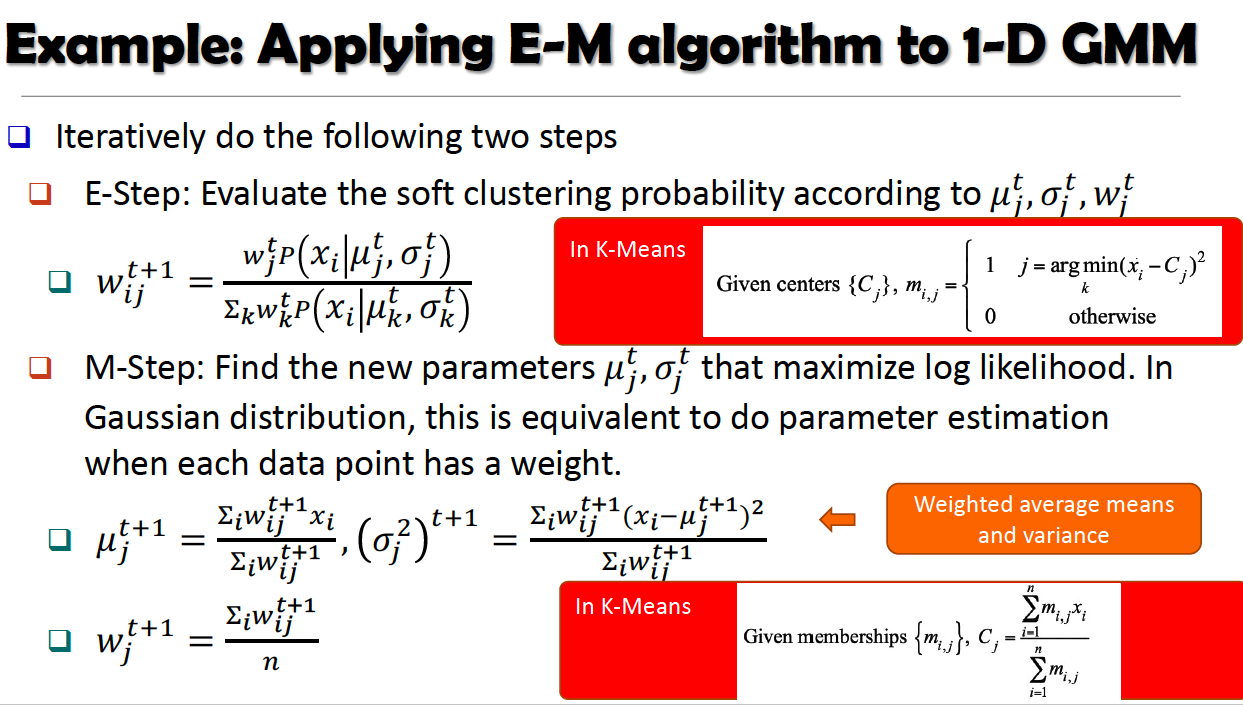
\includegraphics[width=0.8\linewidth]{fig/gmm.png}
\end{figure}

\textbf{Pros}: more general than partitioning (different densities and cluster sizes); cluster can be characterized by a small number of parameters; results satisfy statistical assumptions 
\textbf{Cons}: local minimal (solve by repeat running and random initialize); computationally expensive, hard to estimate \# of clusters; only deal with spherical cluster

Mixture model for doc clustering: a set of language model $\Theta={\theta_1,\dots,\theta_k}$, where $\theta_i=\{p(w_1|\theta_i),\dots,p(w_v|\theta_i)\}$. Prob $p(d=d_i)=\sum_{\theta_j}p(\theta=\theta_j)p(d=d_i|\theta=\theta_j)\varpropto \sum_{\theta_j}p(\theta=\theta_j)\prod_{k=1}^V[p(w_k|\theta_j)]^{tf(w_k,d_i)}$. 

\textbf{E-step}: $E[z_{ij}]=p(\theta=\theta_j|d=d_i)=\frac{p(d=d_i|\theta=\theta_j)p(\theta=\theta_j)}{\sum_{n=1}^kp(d=d_i|\theta=\theta_n)p(\theta=\theta_n)}=\frac{\prod_{k=1}^V[p(w_k|\theta_j)]^{tf(w_k,d_i)}p(\theta=\theta_j)}{\sum_{\theta_j}\prod_{k=1}^V[p(w_k|\theta_n)]^{tf(w_k,d_i)}p(\theta=\theta_n)}$, where K: \# of clusters, V: \# of terms; N:\# of docs. 

\textbf{M-step}: $p(w_i|\theta_j)=\frac{\sum_{k=1}^NE[z_{kj}]tf(w_i,d_k)}{\sum_{k=1}^NE[z_{kj}]|d_k|}$ and $p(\theta=\theta_j)=\frac{1}{N}\sum_{i=1}^NE[z_{ij}]$


% \end{multicols}
\end{document}